% Enable warnings about problematic code
\RequirePackage[l2tabu, orthodox]{nag}

\documentclass{WeSTassignment}

% The lecture title, e.g. "Web Information Retrieval".
\lecture{Introduction to Web Science}
% The names of the lecturer and the instructor(s)
\author{%
  Prof. Dr.~Steffen~Staab\\{\normalsize\mailto{staab@uni-koblenz.de}} \and
  Ren{\'e}~Pickhardt\\{\normalsize\mailto{rpickhardt@uni-koblenz.de}} \and
   Korok~Sengupta\\{\normalsize\mailto{koroksengupta@uni-koblenz.de}}
}
% Assignment number.
\assignmentnumber{6}
% Institute of lecture.
\institute{%
  Institute of Web Science and Technologies\\%
  Department of Computer Science\\%
  University of Koblenz-Landau%
}
% Date until students should submit their solutions.
\datesubmission{December 6, 2016, 10:00 a.m.}
% Date on which the assignments will be discussed in the tutorial.
\datetutorial{December 9, 2016, 12:00 p.m.}

% Set langauge of text.
\setdefaultlanguage[
  variant = american, % Use American instead of Britsh English.
]{english}

% Specify bib file location.
\addbibresource{bibliography.bib}

% For left aligned centerd boxes
% see http://tex.stackexchange.com/a/25591/75225
\usepackage{varwidth}

% ==============================================================================
% Document

\begin{document}

\maketitle
Please look at the lessons 1) \textbf{Simple descriptive text models} \& 2) \textbf{Advanced descriptive text models}

For all the assignment questions that require you to write code, make sure to include the code in the answer sheet, along with a separate python file. Where screen shots are required, please add them in the answers directly and not as separate files.\\ \\ 

%Please mention your team Names here: 
Team Name: papa
\\Members: Brigitte Aznar
\\ Bonasmitha Behura
\\ Ilia Tugushi

% ------------------------------------------------------------------------------
\section{Digging deeper into Norms (10 points)}

You have been introduced to the concept of a norm and have seen that the uniform norm $|| \cdot ||_\infty$ fullfills all three axioms of a norm which are:

\begin{enumerate}
\item Positiv definite
\item Homogeneous
\item Triangle inequality
\end{enumerate}

Recall that for a function $f:M\longrightarrow \mathbb{R}$ with $M$ being a finite set\footnote{You could for example think of the function measuring the frequency of a word depening on its rank.} we have defined the $L_1$-norm of $f$ as:

\begin{equation}
|| f ||_1 := \sum_{x\in M}|f(x)|
\end{equation}

In this exercise you should
\begin{enumerate}
\item calculate $||f - g||_1$ and $||f -g||_\infty$ for the functions $f$ and $g$ that are defined as \begin{itemize}
\item $f(0) = 2, f(1) = -4, f(2) = 8, f(3) = -4$ and 
\item $g(0) = 5, f(1) = 1, g(2) = 7, g(3) = -3$ \end{itemize}
for: $||f - g||_\infty$
\\$||2 - 0|| = 2$
\\$||-4 - 1|| = 5$
\\$||8 - 7|| = 1$
\\$||-4 + 3|| = 1$

For the given values of f and g  $||f - g||_\infty$ = \textbf{5}
\\\\for: $||f-g||_1$
\\ $\sigma ||f-g||_\infty$
\\ $2 + 5 + 1 + 1 = 9$
\item proof that all three axioms for norms hold for the $L_1$-norm.

Positive definitive:
\\ $||f||_1 = \Sigma|f(x)|$
\\ $||f||_1 = 0 <=> \Sigma |f(x)| = 0$
\\ $|f(x)| = 0 ∀x => f = 0$

Homogeneous
\\$||αf||_1 = α||f||_1$
\\$α||f||_1 = \Sigma |α·f|$
\\$\Sigma |α·f|_1 = \Sigma |α|·|f|$
\\$\Sigma |α|·|f| = |α|\Sigma|f|$
\\$|α|\Sigma|f| = α·||f||_1$

Triangle inequity
\\$||f+g||_1 \leq ||f||_1 + ||g||_1$
\\$||f+g||_1 \leq \Sigma |f+g|$
\\$||f+g||_1 \leq \Sigma |f| + |g|$
\\$||f+g||_1 \leq \Sigma|f| + \Sigma |g|$
\\$||f+g||_1 \leq ||f||_1 + ||g||_1$
\\$||f+g||_1 \leq ||f + g||_1$
\end{enumerate}

\subsection{Hints:}
\begin{enumerate}
\item The proofs work in a very similar fashion to those from the uniform norm that was depicted in the videos. 

\item You can expect that the proofs for each property also will be "three-liners".

\item Both parts of this exercise are meant to practice proper and clean mathematical notation as this is very helpfull when reading and understanding research papers. Discuss in your study group not only the logics of the calculation and the proof (before submission) but try to emphasize on the question whether your submission is able to communicate exactly what you are doing. 

\end{enumerate}



% ------------------------------------------------------------------------------
\section{Coming up with a research hypothesis (12 points)}
You can find all the text of the articles from Simple English Wikipedia at \url{http://141.26.208.82/simple-20160801-1-article-per-line.zip} each line contains one single article. 

In this task we want you to be creative and do some research on this data set. The ultimate goal for this exercise is to practice the way of coming up with a research hypothesis and testable predictions. 

In order to do this please \textbf{shortly}\footnote{Depending on the question shortly could mean one or two sentences or up to a thousand characters. We don't want to give a harsh limit because we trust in you to be reasonable.} answer the following questions: 

\begin{enumerate}
\item What are some observations about the data set that you can make? State at least three observations.
\begin{enumerate}
\item 7 out of the 10 first articles have the Word "is" as the 2nd word of the articles.
\item Simple English Wikipedia has short articles.
\item Most of the articles contain less than 15 sentences.
\end{enumerate}
\item Which of these observations make you curious and awaken your interest? Ask a question about why this pattern could occur.
\\ \texttt{"Simple English Wikipedia has short articles"}
\\ Can it be read in a short amount of time?
\item Formulate up to three potential research hypothesis.
\begin{enumerate}
\item \texttt{It's possible to read Simple English Wikipedia in 30 days.}
\\ It may take longer to read, based on the number of words and the avg human reading speed.
\item \texttt{More than 50 \% of the articles in Simple English Wikipedia have less than 15 sentences.}
\\Count the number of sentences and then calculate the percentage of articles for which this is true.
\end{enumerate}

\item Take the most promising hypothesis and develop testable predictions.
\\ \texttt{It's possible to read Simple English Wikipedia in a 30 days time.}

\item Explain how you would like to use the data set to test the prediction by means of descriptive statistics. Also explain how you would expect your outcome. 
\begin{enumerate}
\item Count all the words in the data set by using regular expression (r'\textbackslash w+'). Being a word (consecutive alphanumeric characters)
\item Calculate how much time does an average reader needs to read the entire data set
\item Calculate how much time does a speedy reader needs to read the entire data set
\end{enumerate}

(If you realize that the last two steps would not lead anywhere repeat with one of your other research hypothesis.)
\end{enumerate}

\subsection{Hints:}
\begin{itemize}
\item The first question could already include some diagrams (from the lecture or ones that you did yourselves).
\item In step 3 explain how each of your hypothesis is falsifiable. 
\item In the fifth step you could state something like: "We expect to see two diagrams. The first one has ... on the x-axis and ... on the y-axis. The image should look like a ... The second diagram ...". You could even draw a sketch of the diagram and explain how this would support or reject your testable hypothesis. 
\end{itemize}

% ------------------------------------------------------------------------------


\section{Statistical Validity (8 points)}
In the above question, you were asked to formulate your hypothesis. In this one, you should follow your own defined roadmap from task 2 validate (or reject) your hypothesis. 

\subsection{Hints:}
\begin{itemize}
\item In case feel uncomfortable to test one of the predictions from task 2 you can "steal" one of the many hypothesis (and with them imlicitly associated testable predictions) or diagrams depicted from the lecture and reproduce it. However in that case you cannot expect to get the total amount of points for task 3. 
\end{itemize}

\begin{lstlisting}

# coding: utf-8

# # It's possible to read Simple English Wikipedia in 30 days time

# Avarage reading speed is 180 Words per minute (in a monitor)
# source: https://en.wikipedia.org/wiki/Words_per_minute#Reading_and_comprehension
# Speed readers can read about 700 words per minute
# source: https://en.wikipedia.org/wiki/Speed_reading
# 
# Given this: Count the total number of words in Simple English Wikipedia
# and calculate how long it will take for each to finish reading it.
# 
# Since the initial observation states that Simple English Wikipedia articles are 
# short, counting this words, and taking this speeds into consideration.
# We calculated that 30 days is a plausible time for doing this task.

# In[43]:

import os
import re
import matplotlib.pyplot as plt
import matplotlib.patches as mpatches


# In[8]:

def get_total_words():
    total_words = 0
    with open("simple-20160801-1-article-per-line\simple_english_wikipedia.txt", encoding="utf8") as file:
        for line in file:
            total_words += len(re.findall(r'\w+', line))
    return total_words


# In[9]:

def get_avg_time(words):
    avg_speed = 180
    return ((words/avg_speed)/60)/24
    
    


# In[10]:

def get_speedy_time(words):
    speedy_speed = 700
    return ((words/speedy_speed)/60)/24
    


# In[11]:

def get_wpm(words):
    time = 43200 #30 days in minutes
    return (words/time)


# In[12]:

words       = get_total_words()
avg_time    = get_avg_time(words)
speedy_time = get_speedy_time(words)

print("Total number of words: ", words)
print("Total time (in days) for an average reader: ", round(avg_time,2))
print("Total time (in days) for a speed reader: ", round(speedy_time,2))


# It is not possible to read simple english wikipedia within 30 days (for a normal reader)
# However it is possible to do it for a speed reader.

# In[14]:

wpm = get_wpm(words)
print("In order to be able to read single english wikipedia within 30 days, a person should read at least", round(wpm,2), "words per minute")


# In[54]:

y = [round(avg_time, 2),round(speedy_time,2)]
x = len([round(avg_time, 2),round(speedy_time,2)])
width = 1/1.5
plt.bar(1, round(avg_time, 2), width, color="blue")
plt.bar(2, round(speedy_time,2), width, color="red")
plt.ylabel('Time in days')
plt.xlabel('Readers')


avg_reader = mpatches.Patch(color='blue', label='Averge reader')
speedy_reader = mpatches.Patch(color='red', label='Speed reader')

plt.legend(handles=[avg_reader, speedy_reader],loc=5)
plt.show()

\end{lstlisting}

According to our findings, it is not possible to read Simple English Wikipedia in 30 days for an average reader. However it is possible for a speed reader to accomplish this task\
In the following plot, we can see how the two types of reader compare to each other.

\begin{figure}[h]
  \centering
  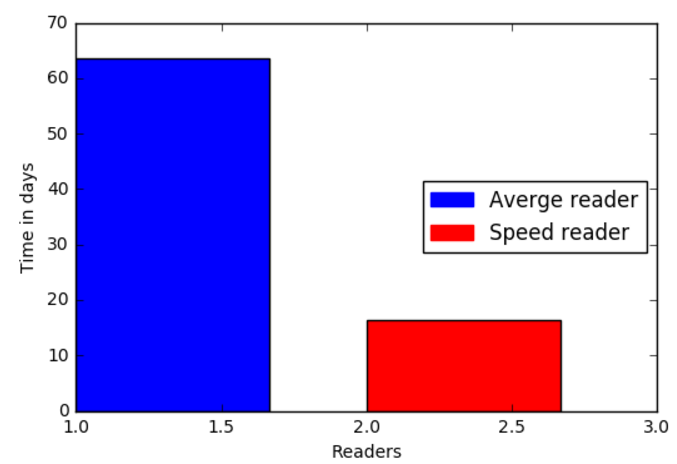
\includegraphics{plot.png}
   \caption{Shows difference in time between average reader and speed reader}
     \label{fig:dig} 
\end{figure}

% ------------------------------------------------------------------------------






\makefooter

\end{document}
